Figure~\ref{fig:words-sentence} compares the generated corpora against Ausonius' own \textit{Cento Nuptialis} along two lexical axes: raw length (words per cento) and syntactic rhythm (mean words per sentence, sentences delimited by strong punctuation). Both RQ2 (exact morae match) and RQ3 (split-pattern match only) reproduce near-identical, tightly clustered distributions ($856.9\pm10.8$ and $861.2\pm11.0$ words respectively; $16.59\pm1.95$ and $16.64\pm2.03$ words/sentence), confirming that relaxing the morae constraint from RQ2 to RQ3 does not measurably change either statistic. The gold cento, however, sits outside both word-count distributions entirely (893 words, roughly three standard deviations above either mean), while its sentence length (17.5 words/sentence) falls comfortably within the generated spread. This split is informative: the skeleton-preserving generation procedure (fixed line/segment/continuation structure) reliably reproduces Ausonius' syntactic pacing, but the free lexical substitution at each slot tends to draw shorter Vergilian fragments on average, so the reconstructed poems run consistently shorter than the original despite sharing its sentence rhythm.

\begin{figure}[htbp]
    \centering
    \begin{subfigure}[b]{0.48\textwidth}
        \centering
        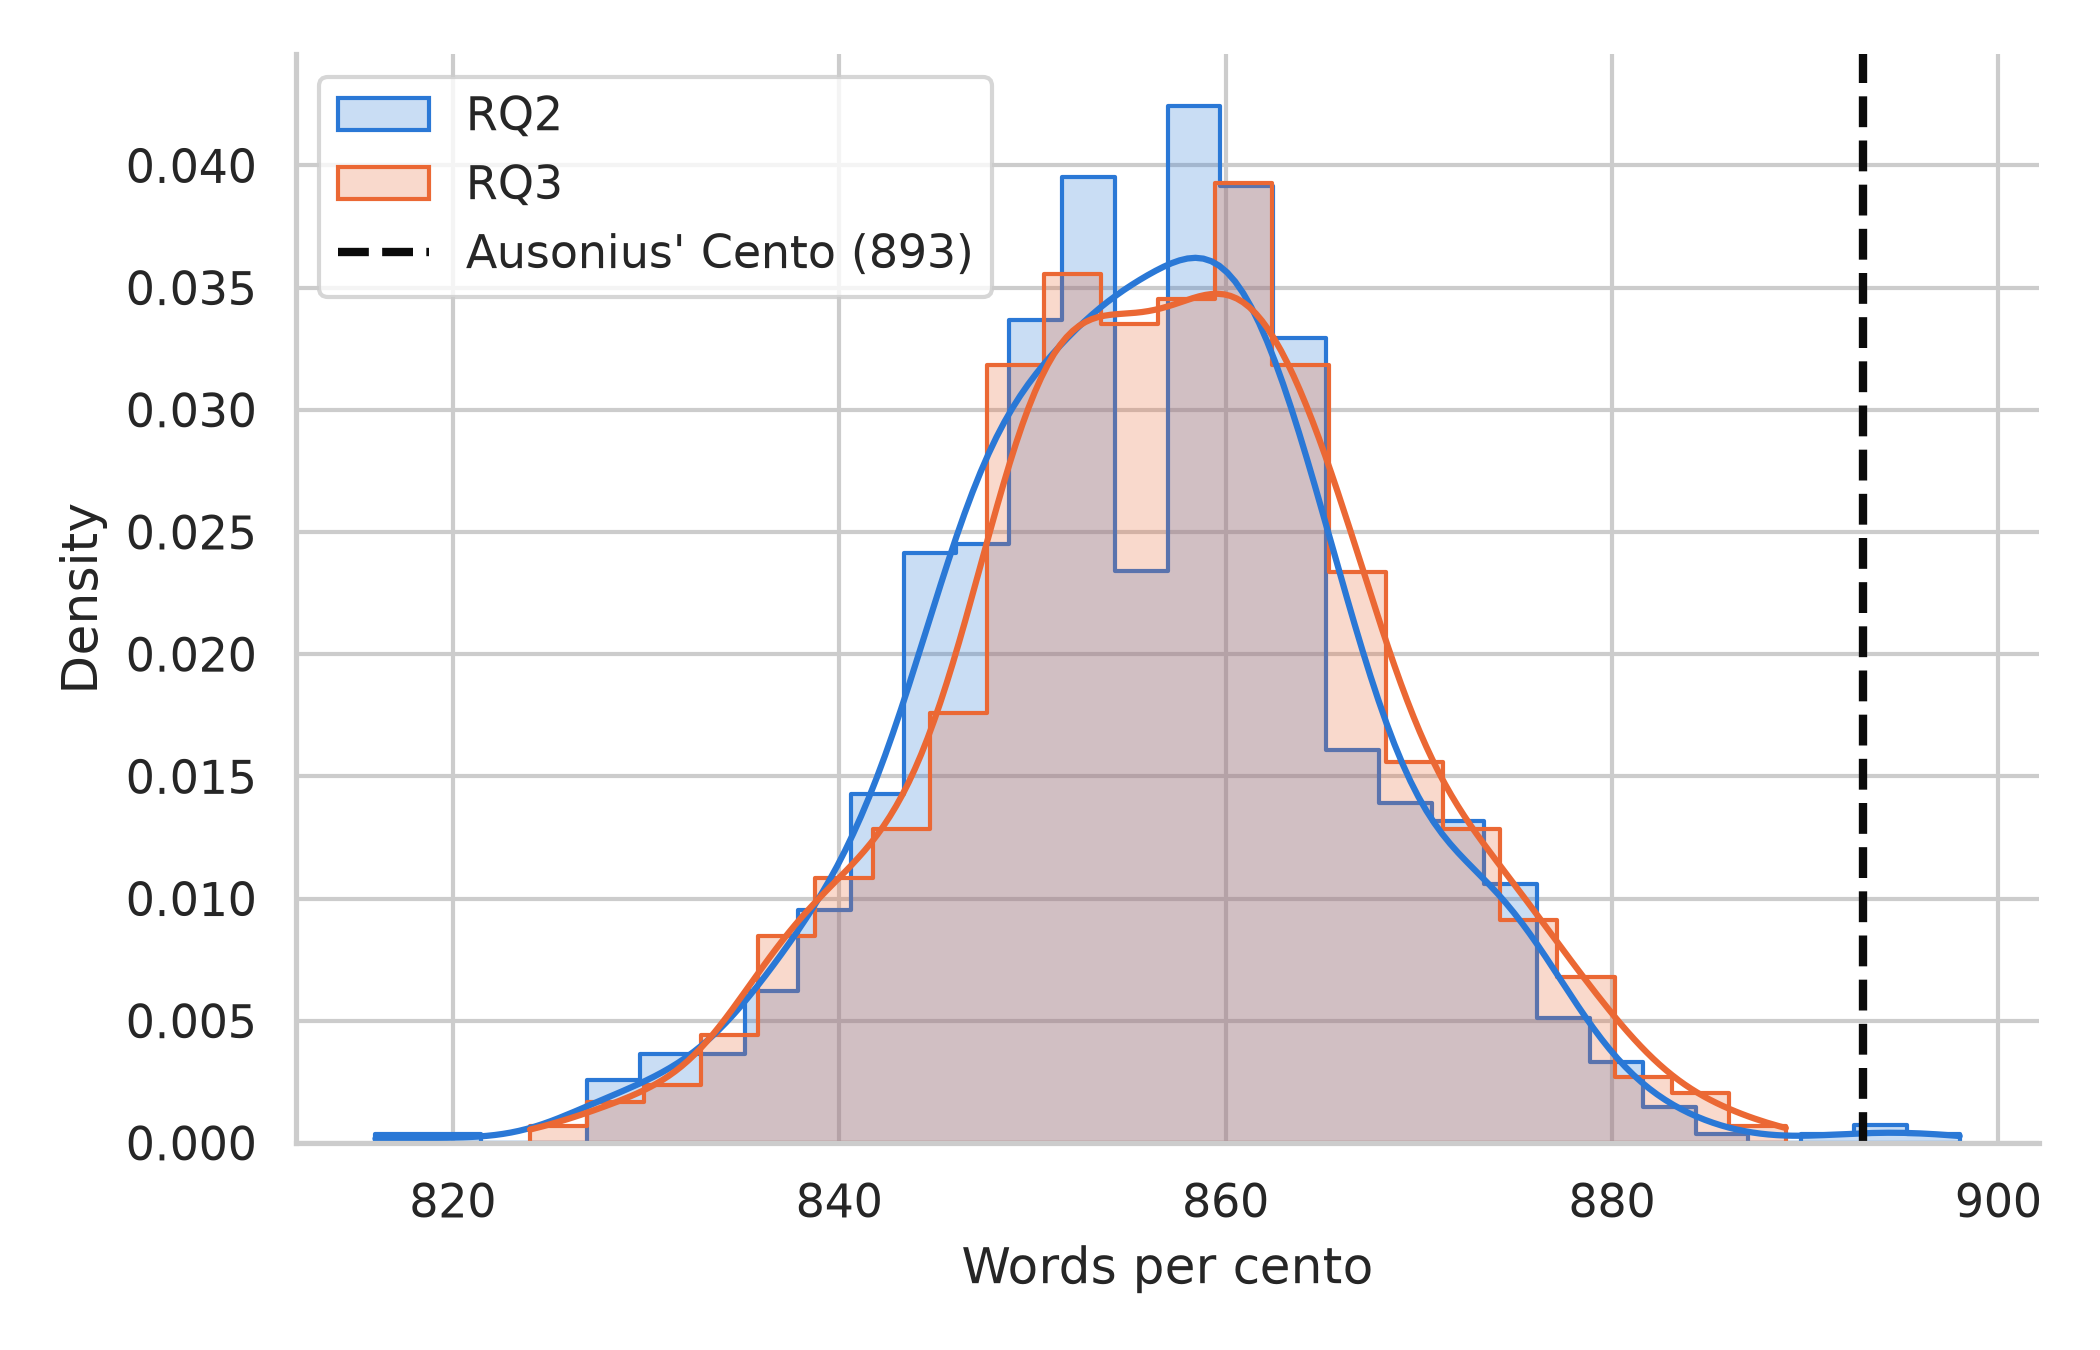
\includegraphics[width=\textwidth]{words_per_cento.png}
        \caption{Words per cento}
        \label{fig:words-per-cento}
    \end{subfigure}
    \hfill
    \begin{subfigure}[b]{0.48\textwidth}
        \centering
        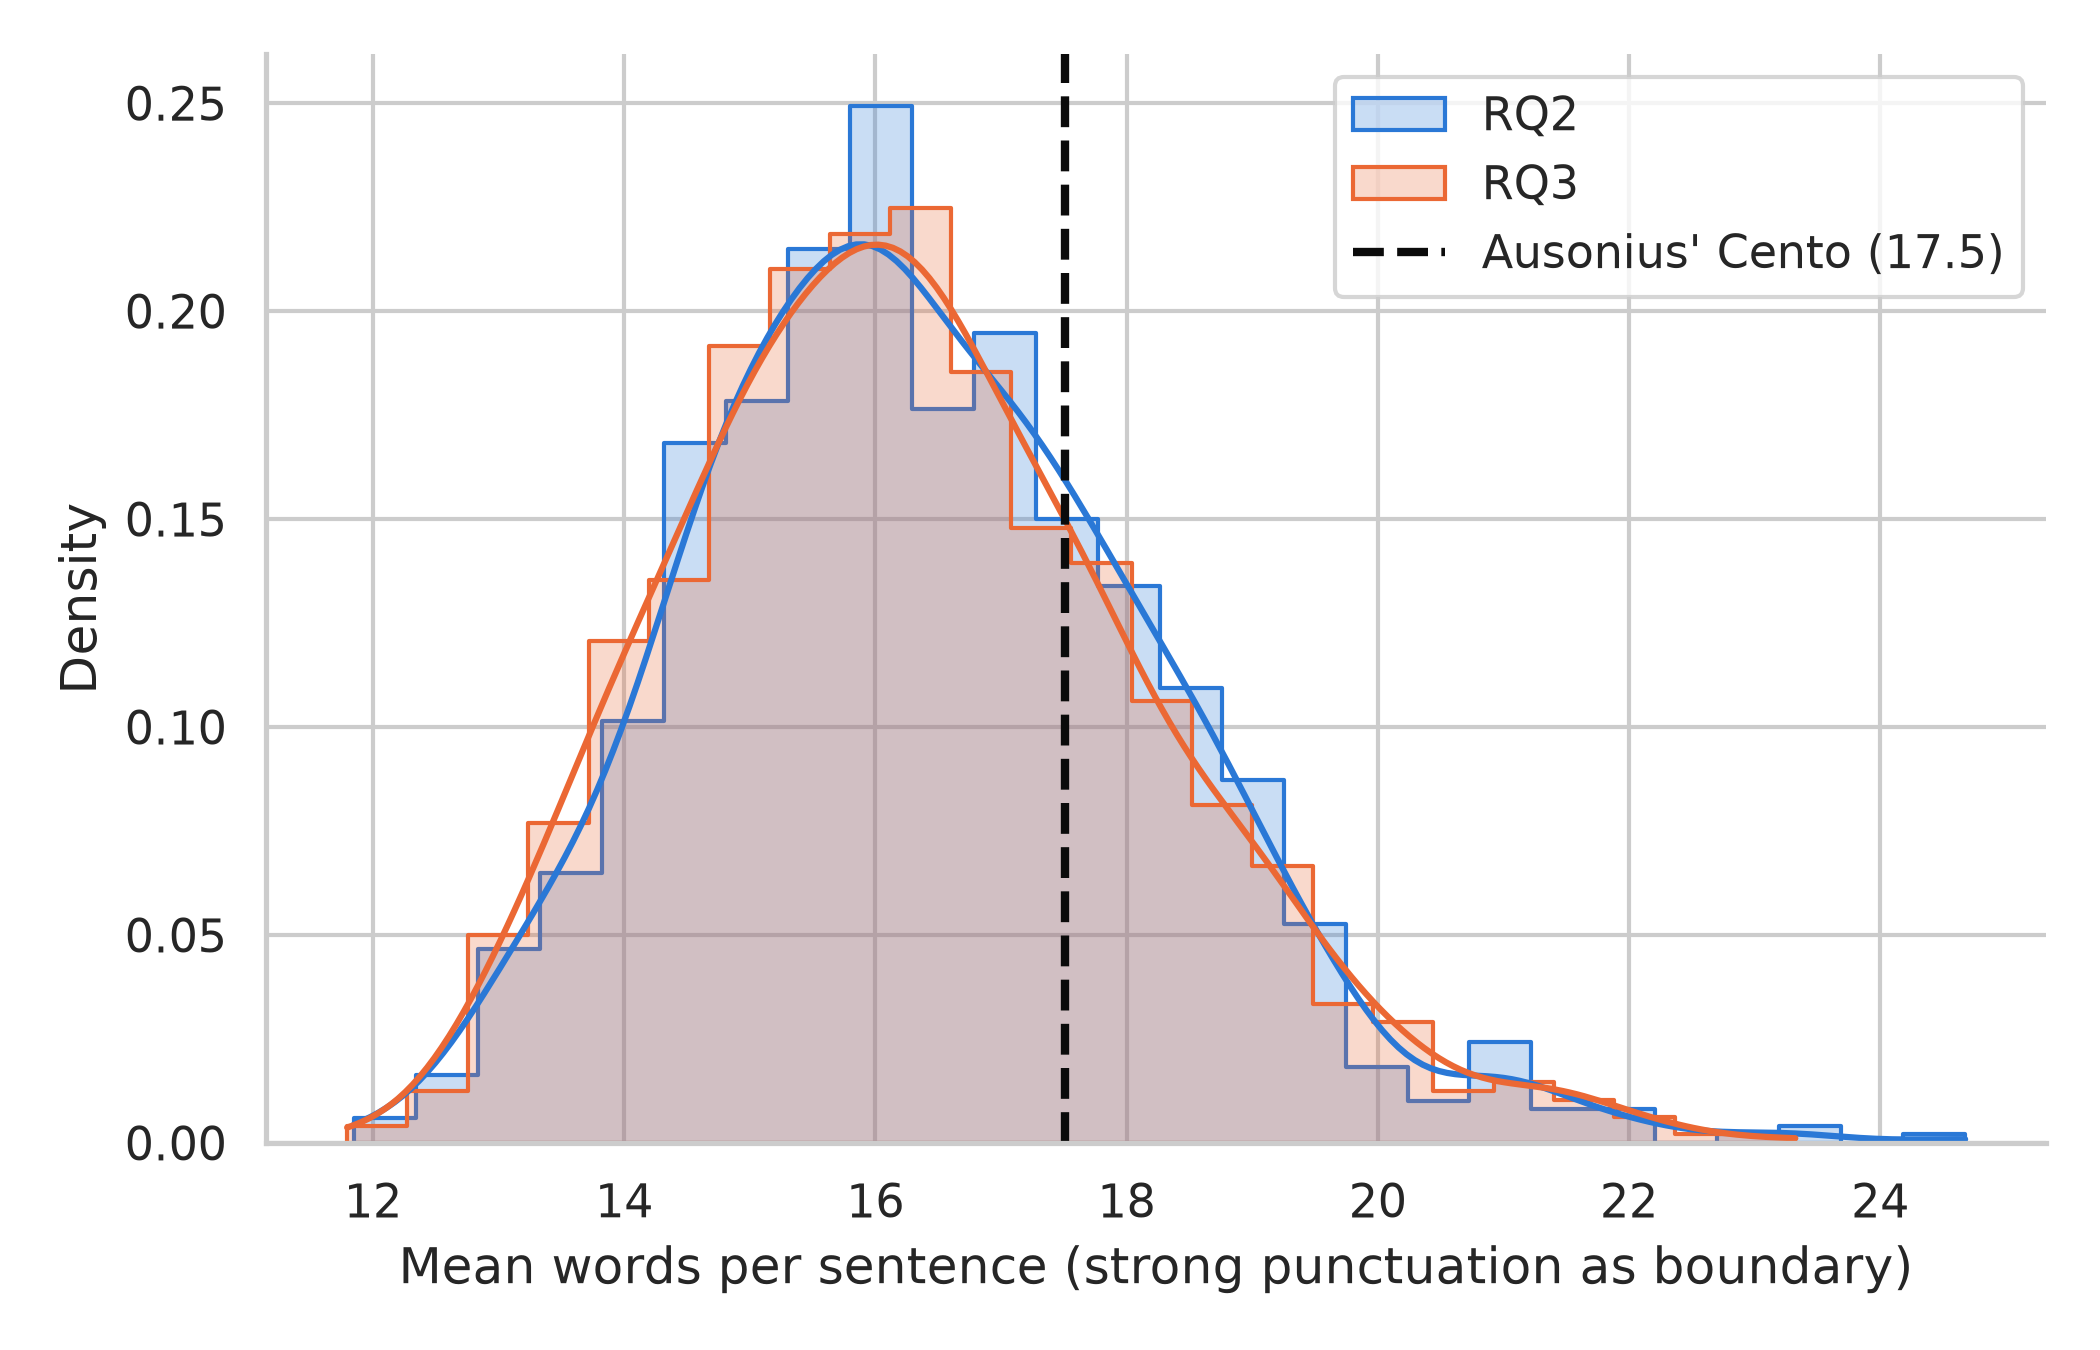
\includegraphics[width=\textwidth]{sentence_length_per_cento.png}
        \caption{Mean words per sentence}
        \label{fig:sentence-length-per-cento}
    \end{subfigure}
    \caption{Distributions of words per cento (left) and mean sentence length (right) across the 1000-poem RQ2 and RQ3 corpora, with Ausonius' own \textit{Cento Nuptialis} shown as a dashed reference line.}
    \label{fig:words-sentence}
\end{figure}
